\documentclass[notitlepage,11pt]{report}

\input{../Header.tex}
\tikzstyle{class}=[rectangle, draw=black, fill=white, rounded corners, drop shadow, text centered, anchor=north, text width=5cm]
\geometry{left=1in, right=1in, top=1in, bottom=0.8in}

\graphicspath{{../assignment3/UI/}}

\title{Activity 9}
\author{Tripp Isbell\\
	\texttt{cai0004@auburn.edu}}
\date{}

\begin{document}
\maketitle
3-tier:
\begin{itemize}
	\item User Interface
	\begin{itemize}
		\item MainView: main menu
		\begin{figure}[h] 
			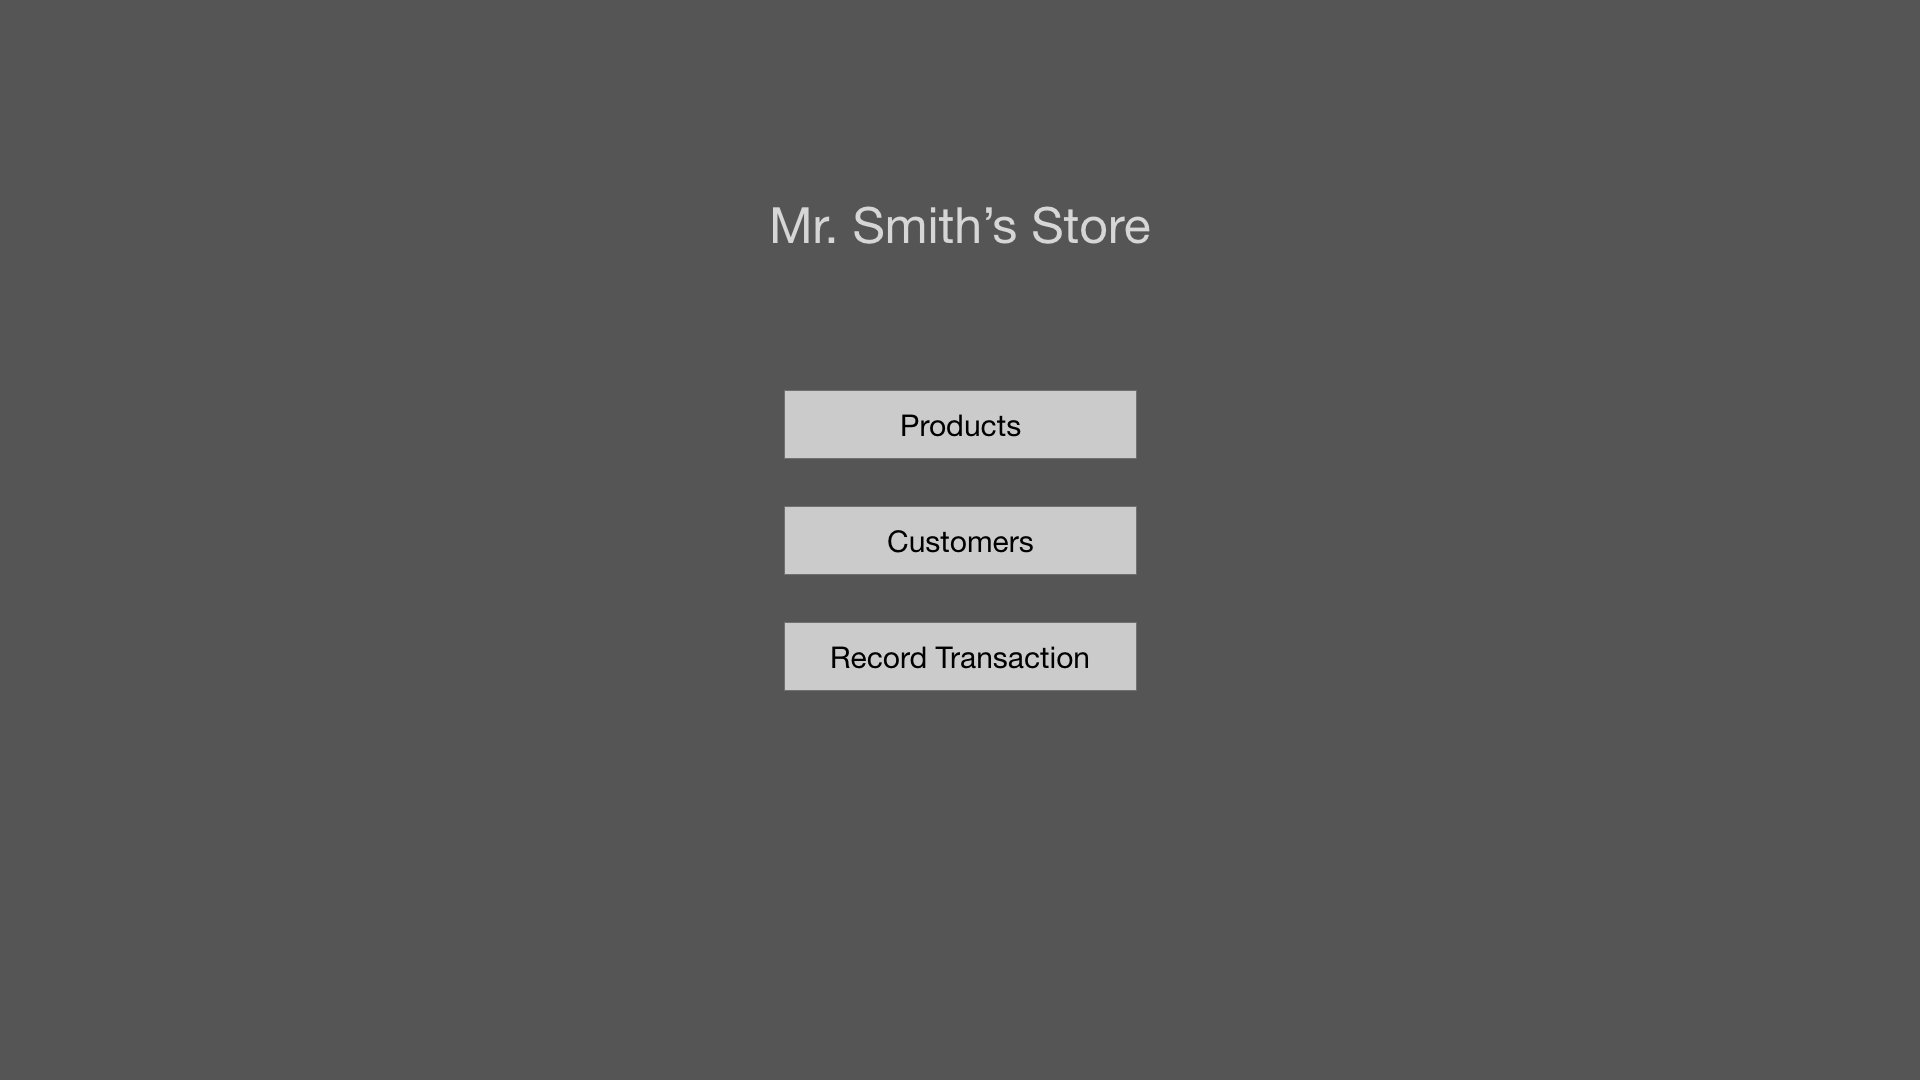
\includegraphics[scale=0.12]{MainMenu}
		\end{figure}
		\item ProductsView: products database
		\begin{figure}[h]
			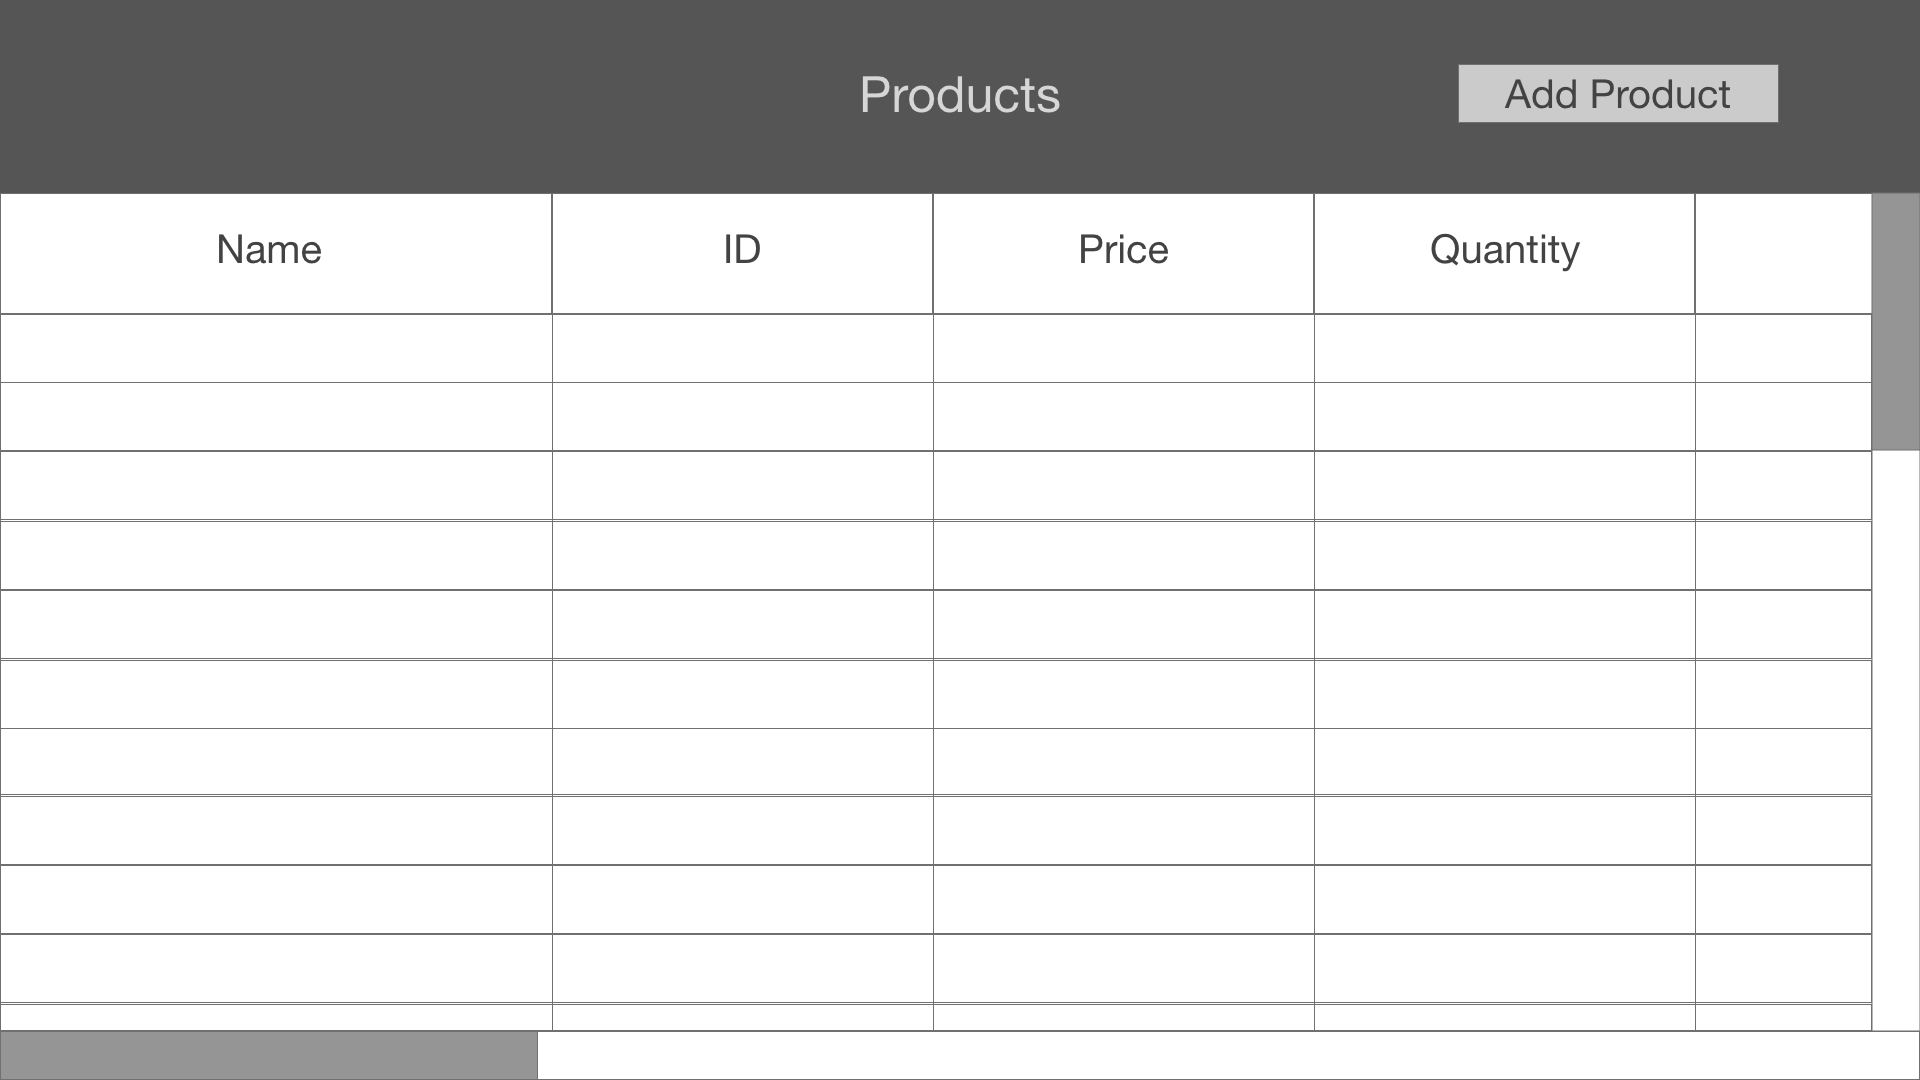
\includegraphics[scale=0.12]{AddProduct}
		\end{figure}
		\item AddProductView 
		\begin{figure}[h]
			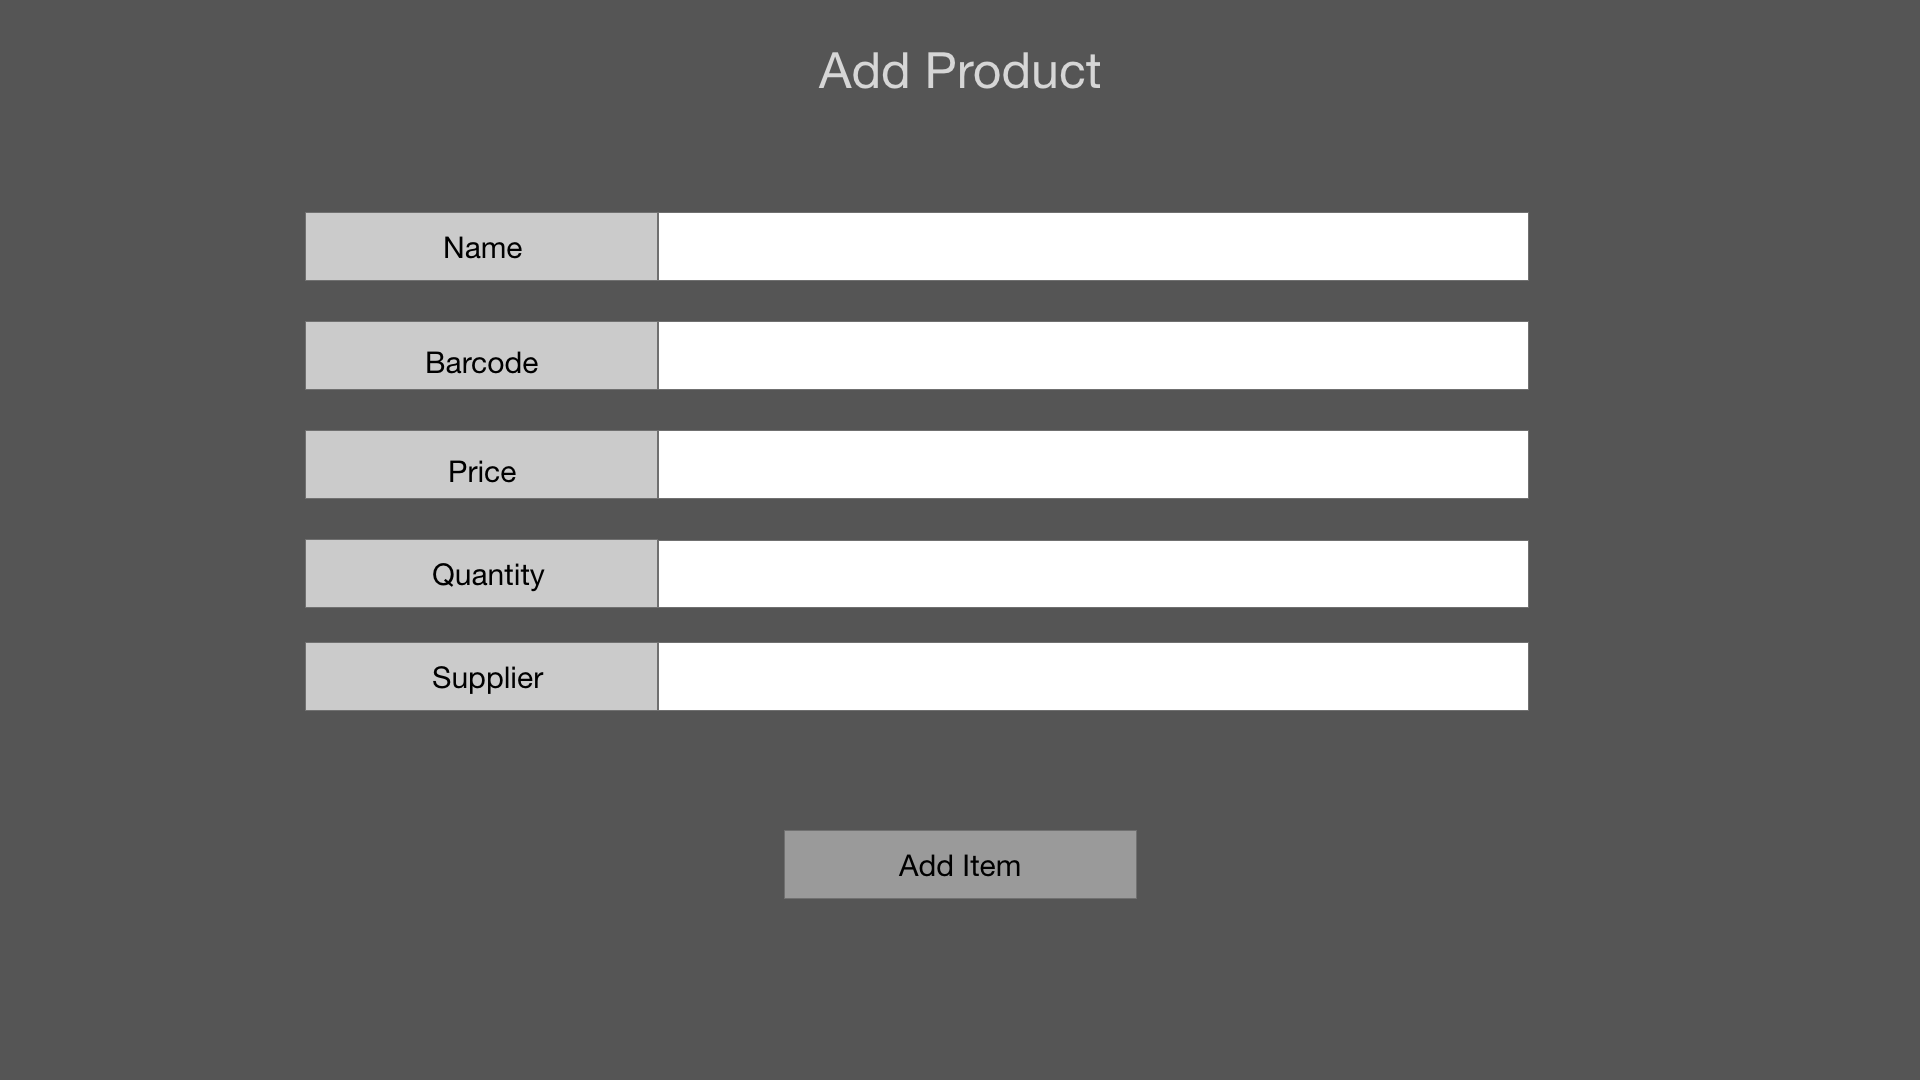
\includegraphics[scale=0.12]{ProdInfo}
		\end{figure}
		\newpage
		\item CustomersView: customers database
		\begin{figure}[h]
			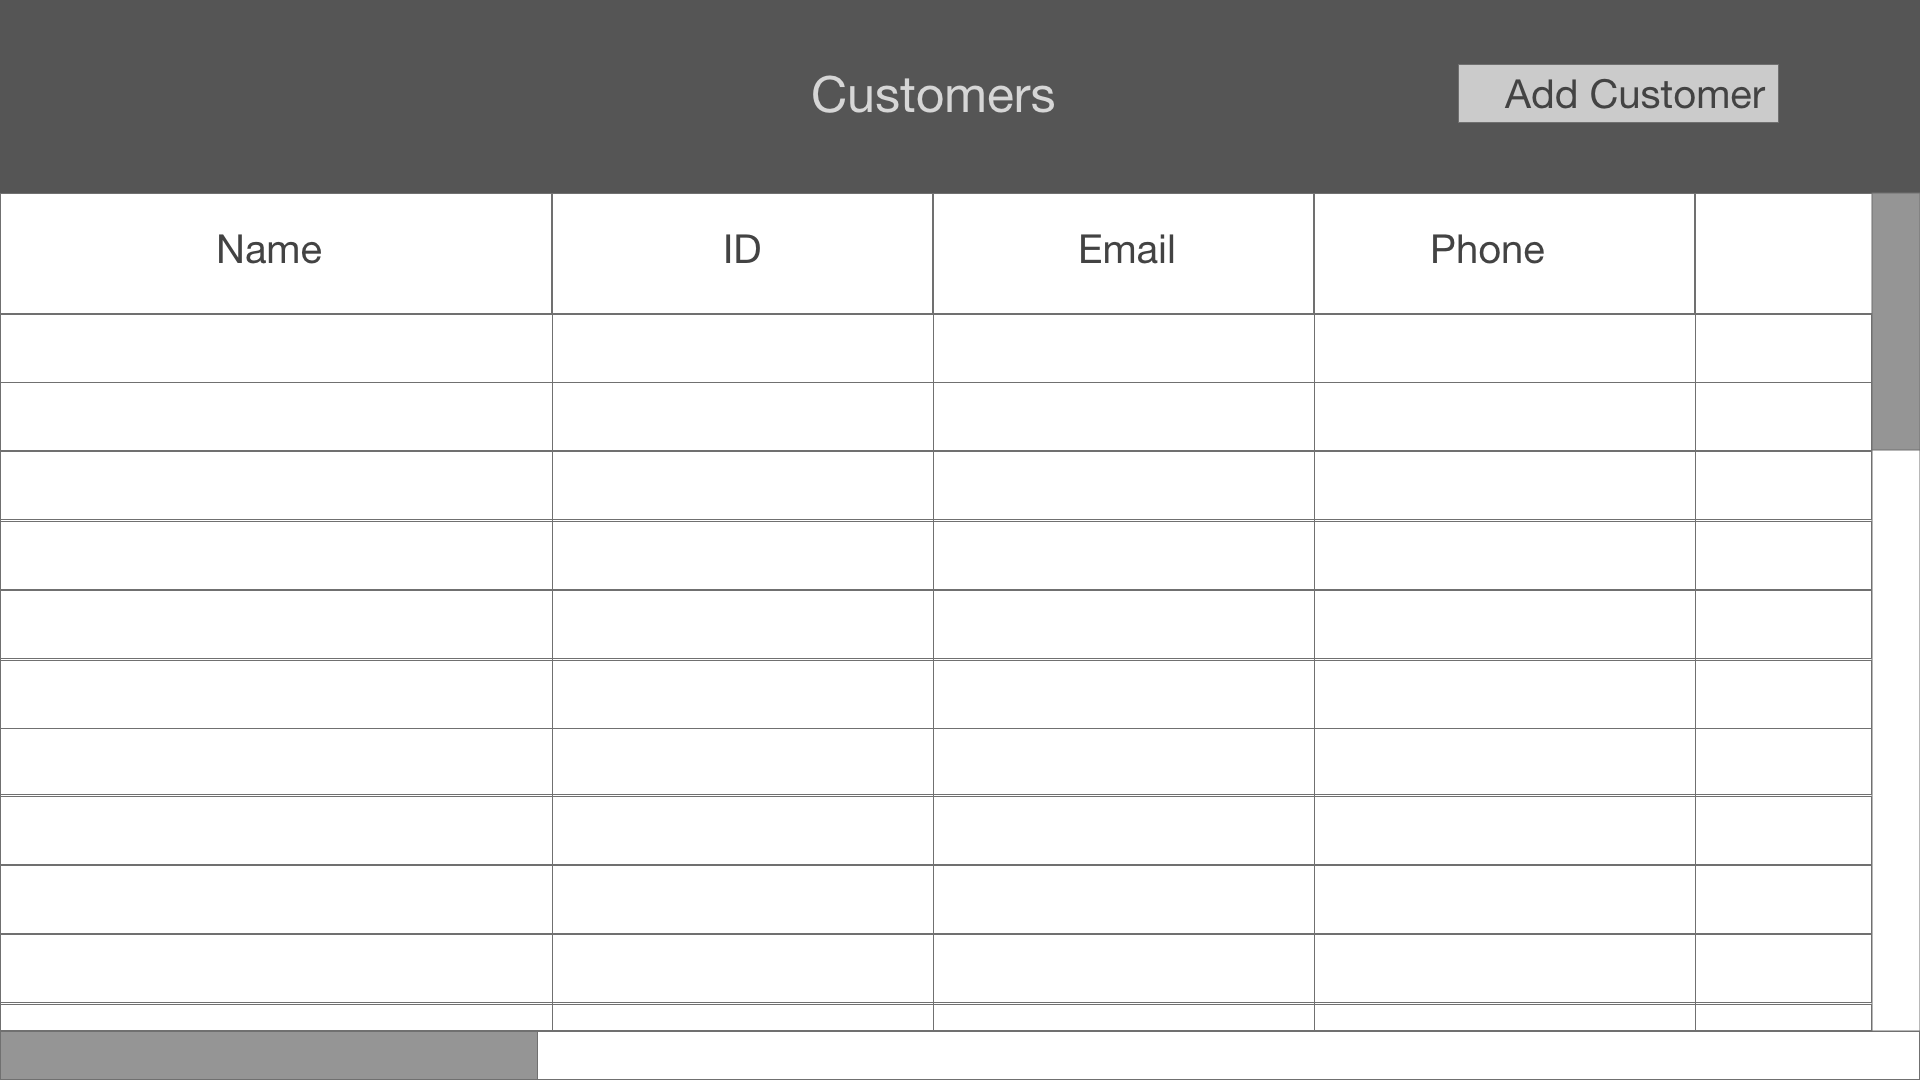
\includegraphics[scale=0.12]{AddCustomer}
		\end{figure}
		\item AddCustomerView 
		\begin{figure}[h]
			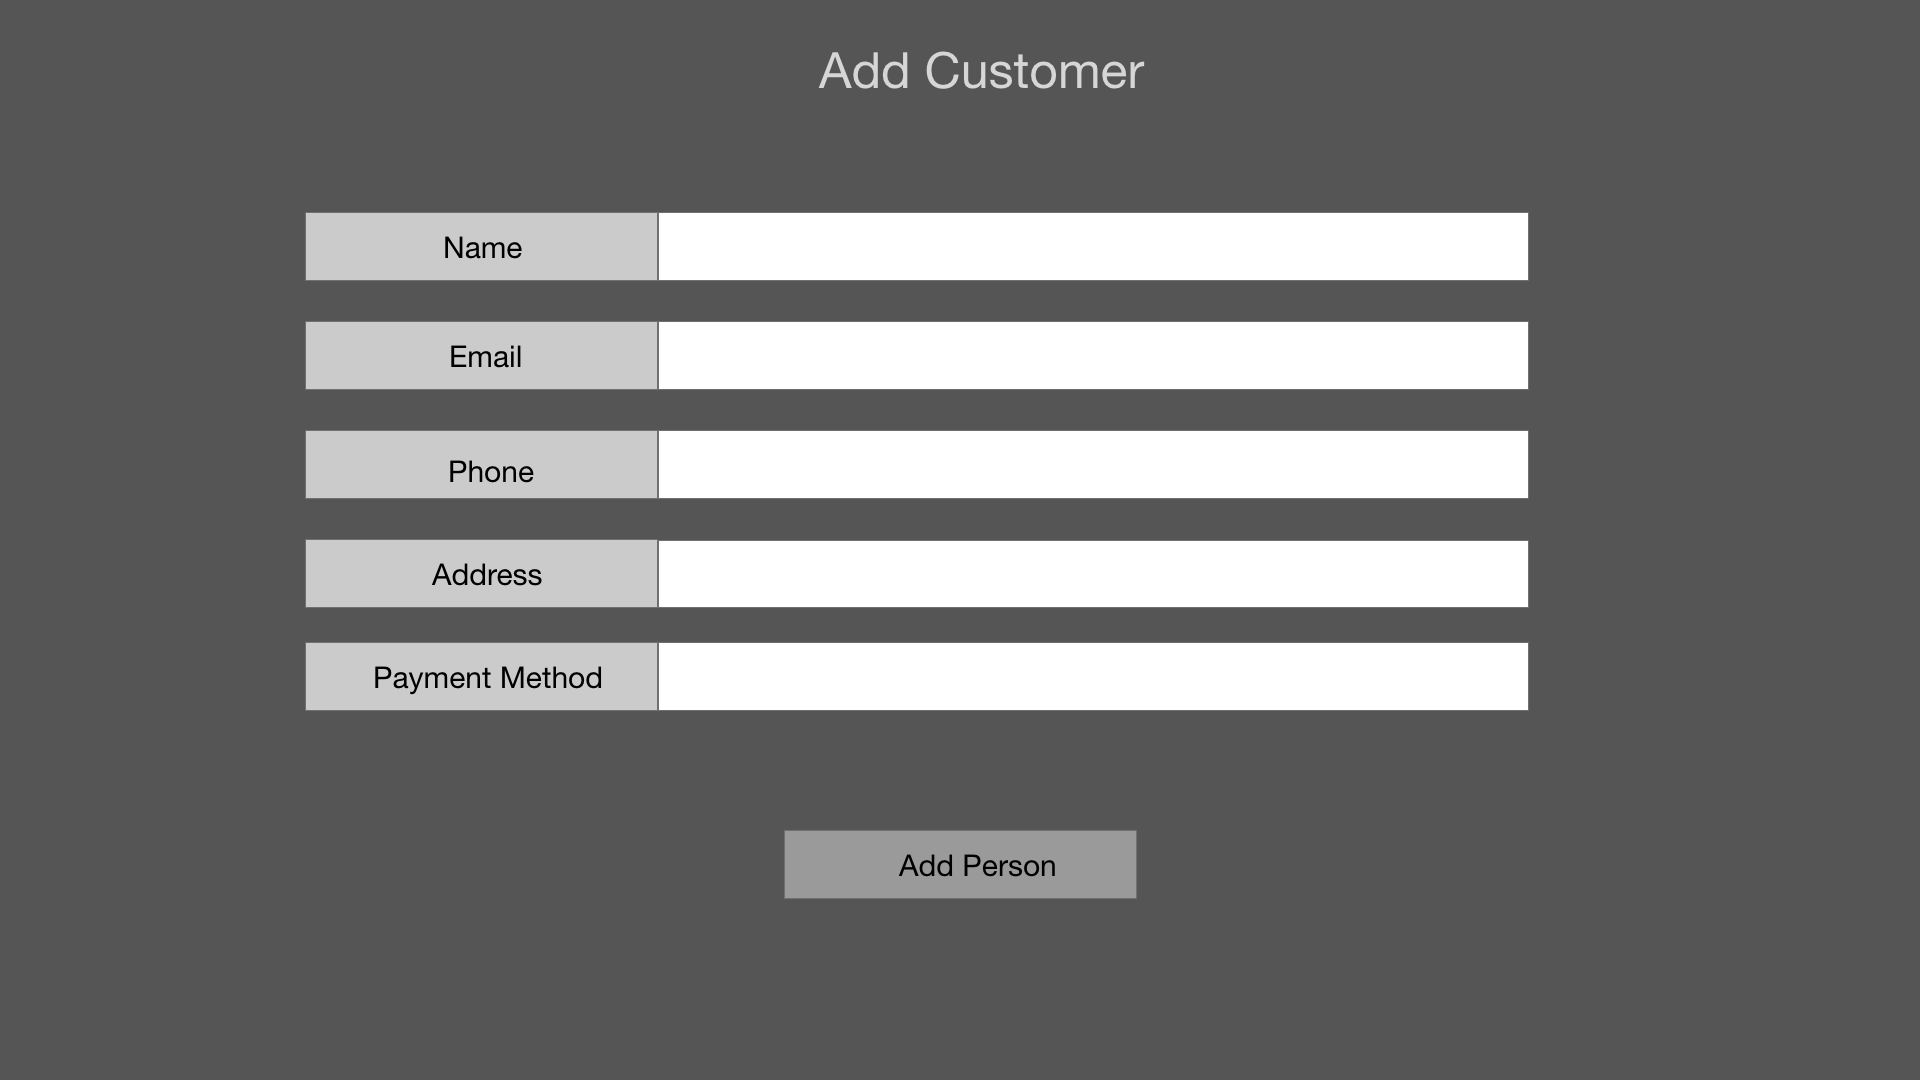
\includegraphics[scale=0.12]{CustInfo}
		\end{figure}
	\end{itemize}
	\item Business Logic
	\begin{itemize}
		\item ProductModel: store information of product
		\item CustomerModel: store information of a customer
		\item AddProductController: process events of AddProductView
		\item ProductsViewController
		\item StoreManager: main application object
		\item Application
	\end{itemize}
	\item Data Access
	\begin{itemize}
		\item SQLiteDataAdapter: read/write data
		\item SQLite database
	\end{itemize}
\end{itemize}
\begin{center}
\begin{tikzpicture}
	\node (Controller) [class]
		{
		Controller\\
		AddProductsController\\
		MainViewController\\
		ProductsViewController\\
		CustomersViewController\\
		AddCustomerViewController
		};
	\node (Model) [class, right=0.5in of Controller] 
		{
		Model\\
		ProductModel\\
		CustomerModel
		} edge[<->] (Controller);
	\node (View) [class, left=0.5in of Controller] 
	{
		View\\
		MainView\\
		ProductsView\\
		AddProductView\\
		CustomersView\\
		AddCustomerView	
	} edge[<->] (Controller);
\end{tikzpicture}
\end{center}
\end{document}